\documentclass[10pt, letterpaper]{article}
\usepackage{setspace}
\usepackage[letterpaper, margin=1.0in]{geometry}
\addtolength{\topmargin}{-0.25in}
%\usepackage{tocloft}
\usepackage{titlesec}
%\titleformat*{\section}{\large\bfseries}
\titleformat*{\section}{\large}
\titleformat*{\subsection}{\normalsize}
\usepackage{enumitem}
\usepackage{listings}
\usepackage{amsmath}   % includes \boldmath(), \boldsymbol{()}
\usepackage{bm}        % math fonts, \boldmath{}, \boldsymbol{}
\usepackage{graphicx}
\usepackage{float}
\graphicspath{{images/}}
\usepackage{subcaption}
\usepackage{xcolor, colortbl}
\definecolor{gray}{gray}{0.9}
\definecolor{ltBlue}{rgb}{0.75, 0.85, 0.975}
\definecolor{medBlue}{rgb}{0.75, 0.8, 0.9}
\definecolor{white}{rgb}{1, 1, 1}
%\rowcolor{ltBlue}
\usepackage{changepage}
\usepackage{pdflscape}
\bibliographystyle{plainnat}
\usepackage[authoryear, round, semicolon]{natbib}
\newcommand{\mt}[1]{\bm{#1}^{\prime}}
\newcommand{\mtm}[2]{\bm{#1}^{\prime}\bm{#2}}
\newcommand{\mi}[1]{\bm{#1}^{-1}}
\newcommand{\mest}[1]{\hat{\bm{#1}}}
\usepackage[bottom]{footmisc}
\setlength{\skip\footins}{12pt}
\setlength\parindent{0pt}
%\usepackage{breakurl}
\usepackage{url}
\usepackage{hyperref}
\hypersetup{
    colorlinks=true,
    linkcolor=blue,
    urlcolor=blue,
}
% Disable section numbers, so that hyperlinks are enabled
%\setcounter{secnumdepth}{0}

\title{\Large Co-lab Shiny Workshop\\[6pt]
       \large Session 3, Integrating Shiny and \texttt{visNetwork}\\[6pt]
       April 21, 2021\\[20pt]
       \normalsize thomas.balmat@duke.edu\\[1pt]rescomputing@duke.edu}

%\date{\vspace{-30pt}October 17, 2019}
\date{}
%\author{thomas.balmat@duke.edu\\rescomputing@duke.edu}

\begin{document}
    
\begin{spacing}{1.0}
    
\maketitle

\vspace{-20pt}

%%%%%%%%%%%%%%%%%%%%%%%%%%%%%%%%%%%%%%%%%%%%%%%%%%%%%%%%%%%%%%%%%%%%%%%%%%%%%%%%%%%%%%%%%%%%

A network graph is effective in showing relationships between associated entities.  Entities, or items that are related, are referred to as vertices and the relationships that connect them are referred to as edges.  A graph with many vertices or edges can be very dense, making central features, such as a vertex with many relationships or a particular type of edge that connects many pairs of vertices, difficult to identify.  Iterated adjustment of rendering features, such as the number of vertices displayed, opacity of edges, etc., can aid in presenting a graph that reveals important features of the system being studied, while eliminating ``noisy" relationships that are unrelated to findings of interest.  In this session, we will use the reactive feature of Shiny to develop an app that renders and adjusts a network graph in a genome wide association study (GWAS) pleiotropy setting.  Pleiotropy is a term used to describe the process of comparing significant results from two independent GWAS studies, with the objective of identifying phenotypes (observed traits) in both studies that are correlated with genotypes of a common chromosomal position (these positions are known as single nucleotide ploymorphisms, or SNPs).  The app will produce two styles of graph:  one that generates two sets of phenotype vertices, one from each GWAS, and joins them by common SNP, and another that generates vertices from SNPs that are joined by phenotype.  Implemented features include:

\begin{itemize}[noitemsep]
    \item Phenotype or SNP node filtering by strength of within-GWAS correlation (regression p-value)
    \item Node filtering by number of edges
    \item Selection of phenotype nodes with SNP edges or SNP nodes with phenotype edges
    \item \texttt{visnetWork} ``physics" feature (places nodes using gravitation-like attraction based on mass, or node size)
    \item Edge transparency adjustment
    \item Subnetting of graph by node selection (retains all connected nodes)
    \item Node clustering (collapse of nodes having a specified number of edges into a single node)
    \item Display of a node centrality table
\end{itemize}

%%%%%%%%%%%%%%%%%%%%%%%%%%%%%%%%%%%%%%%%%%%%%%%%%%%%%%%%%%%%%%%%%%%%%%%%%%%%%%%%%%%%%%%%%%%%

\section{Overview}

\begin{itemize}[noitemsep]
    \item Preliminaries
      \begin{itemize}
        \item What can \texttt{Shiny and visNetwork} do for you?
        \item What are your expectations of this workshop?
      \end{itemize}
    \item \hyperref[sec:accesworkshopmaterial]{Download Workshop Material and configure R}
    \item \hyperref[sec:resources]{Resources}
    \item \hyperref[sec:anatomyofapp]{Anatomy of a Shiny App}
    \item \hyperref[sec:reactivity]{Reactivity}
    \item \hyperref[sec:helloVisNetwork]{Hello \texttt{visNetwork}}
    \item \hyperref[sec:visNetwork]{\texttt{visnetwork} Pleiotropy App}
      \begin{itemize}[noitemsep]
        \item \hyperref[sec:visNetworkV1]{Version 1, Basic Network Graph}
        \item \hyperref[sec:visNetworkV2]{Version 2, Enhanced Reactive Graph Controls}
        \item \hyperref[sec:visNetworkV3]{Version 3, Additional Graph Controls with Centrality Table}
      \end{itemize}
    \item \hyperref[sec:UCD]{Integrating \texttt{visNetwork} with a Graph Database for Visual Data Exploration}
    \item \hyperref[sec:altvis]{Alternative Visualizations}
    \item \hyperref[sec:debugging]{Debugging}
\end{itemize}

% Shiny server
% http vs. https
% Global mem

%%%%%%%%%%%%%%%%%%%%%%%%%%%%%%%%%%%%%%%%%%%%%%%%%%%%%%%%%%%%%%%%%%%%%%%%%%%%%%%%%%%%%%%%%%%%%%

%\vspace{0.1in}

\section{Download Workshop Material and Configure R}\label{sec:accesworkshopmaterial}

\begin{itemize}[noitemsep]
    \item Copy course outline, scripts, and data from\\ \url{https://github.com/tbalmat/Duke-Co-lab/tree/master/Spring-2021/Session-4-visNetwork}
    \begin{itemize}[noitemsep]
        \item App.zip
        \item Co-lab-Session-4-visNetwork.pdf
        \item Data.zip
    \end{itemize}
    \item Expand zip files (one subdirectory per file)
    \item Launch RStudio
    \item Install packages:
    \begin{itemize}[noitemsep]
        \item \texttt{install.packages("shiny")}
        \item \texttt{install.packages("shinythemes")}
        \item \texttt{install.packages("visNetwork")}
        \item \texttt{install.packages("DT")}
    \end{itemize}
\end{itemize}

%%%%%%%%%%%%%%%%%%%%%%%%%%%%%%%%%%%%%%%%%%%%%%%%%%%%%%%%%%%%%%%%%%%%%%%%%%%%%%%%%%

\section{Examples}\label{sec:examples}

\begin{itemize}[noitemsep]
  \item \texttt{visNetwork} features:  \url{https://datastorm-open.github.io/visNetwork/}
  \item \texttt{visNetwork} Shiny demo (from within R):  \texttt{shiny::runApp(system.file("shiny", package="visNetwork"))}  \item Delivery graph network app: \url{https://github.com/tbalmat/Duke-Co-lab/tree/master/Examples/GraphDeliveryMap}
  \item Duke University Urea Cycle Disorder exploration app:  \url{https://github.com/tbalmat/Duke-UCD/tree/master/ShinyApp}
  \item Neo4j graph database:  \url{https://neo4j.com/developer/graph-database/}
\end{itemize}


%%%%%%%%%%%%%%%%%%%%%%%%%%%%%%%%%%%%%%%%%%%%%%%%%%%%%%%%%%%%%%%%%%%%%%%%%%%%%%%%%

\section{Resources}\label{sec:resources}

\begin{itemize}

  \item R
    \begin{itemize}   
      \item Books
        \begin{itemize}
          \item Norm Matloff, \textit{The Art of R Programming}, No Starch Press
          \item Wickham and Grolemund, \textit{R for Data Science}, O'Reilly
          \item Andrews and Wainer, \textit{The Great Migration:  A Graphics Novel}, \url{https://rss.onlinelibrary.wiley.com/doi/pdf/10.1111/j.1740-9713.2017.01070.x}
          \item Friendly, \textit{A Brief History of Data Visualization}, \url{http://datavis.ca/papers/hbook.pdf}
        \end{itemize}
      \item Reference cards
        \begin{itemize}
          \item R reference card:  \url{https://cran.r-project.org/doc/contrib/Short-refcard.pdf}
          \item Base R:  \url{https://rstudio.com/wp-content/uploads/2016/10/r-cheat-sheet-3.pdf}
          \item Shiny, \texttt{ggplot}, \texttt{markdown}, \texttt{dplyr}, \texttt{tidy}: \url{https://rstudio.com/resources/cheatsheets/}
        \end{itemize}
    \end{itemize}

  \item Shiny
    \begin{itemize}[noitemsep]
        \item \texttt{?shiny} from the R command line
        \item Click \texttt{shiny} in the \texttt{Packages} tab of RStudio
        \item \url{https://cran.r-project.org/web/packages/shiny/shiny.pdf}
    \end{itemize}

  \item \texttt{visNetwork}
    \begin{itemize}[noitemsep]
        \item \texttt{?visNetwork} from the R command line
        \item Click \texttt{visNetwork} in the \texttt{Packages} tab of RStudio
        \item \url{https://cran.r-project.org/web/packages/visNetwork/visNetwork.pdf}
    \end{itemize}

  \item Workshop materials
    \begin{itemize}
        \item \url{https://github.com/tbalmat/Duke-Co-lab/tree/master/Spring-2021/Session-4-visNetwork}
    \end{itemize}
\end{itemize}

%%%%%%%%%%%%%%%%%%%%%%%%%%%%%%%%%%%%%%%%%%%%%%%%%%%%%%%%%%%%%%%%%%%%%%%%%%%%%%%%%%%%%%%%%%%%%%

\section{Anatomy of a Shiny App}\label{sec:anatomyofapp}

A Shiny app is an R script executing in an active R environment that uses functions available in the Shiny package to interact with a web browser.  The basic components of a Shiny script are

\begin{itemize}
    \item \texttt{ui()} function
    \begin{itemize}
        \item Contains your web page layout and screen objects for inputs (prompt fields) and outputs (graphs, tables, etc.)
        \item Is specified in a combination of Shiny function calls and raw HTML
        \item Defines variables that bind web objects to the execution portion of the app
    \end{itemize}
    \item \texttt{server()} function
    \begin{itemize}
        \item The execution portion of the app
        \item Contains a combination of standard R statements and function calls, such as to \texttt{apply()}, \texttt{lm()}, \texttt{ggplot()}, etc., along with calls to functions from the Shiny package that enable reading of on-screen values and rendering of results
    \end{itemize}
    \item \texttt{runApp()} function
    \begin{itemize}
        \item Creates a process listening on a tcp port, launches a browser (optional), renders a screen by calling the specified \texttt{ui()} function, then executes the R commands in the specified server() function
    \end{itemize}
\end{itemize}

%%%%%%%%%%%%%%%%%%%%%%%%%%%%%%%%%%%%%%%%%%%%%%%%%%%%%%%%%%%%%%%%%%%%%%%%%%%%%%%%%%%%%%%%%%%%%%

\section{Reactivity}\label{sec:reactivity}

Reactivity is the single most important feature that Shiny offers.  Variables are defined in your \texttt{ui()} function with an \texttt{input\$} prefix and when these variables appear in \texttt{observe()} functions within in your \texttt{server()} function, execution events are triggered by on-screen changes to the corresponding \texttt{ui()} variables.  In addition to referencing \texttt{input\$} variables \texttt{observe()} functions include standard R commands, including those supported by any valid R package, so that the reactive variables become parameters to your R functions, enabling dynamic analysis of data.  Output is rendered in the app by targeting \texttt{ui()} variables defined with an \texttt{output\$} prefix.  A simple example follows.  It has a single, numeric input (\texttt{x}) and one plot output (\texttt{plot}).  Changes in \texttt{x} cause the \texttt{observeEvent()} to be executed.  The \texttt{observeEvent()} generates a histogram of \texttt{x} random, normal values.  The histogram is a suitable input value to \texttt{renderPlot()}.  Assignment of the \texttt{renderPlot()} result to \texttt{output\$plot} causes the histogram to be displayed as defined in \texttt{ui()}.  Notice how a Shiny input variable (\texttt{input\$x}) is used as a parameter to an R function (\texttt{rnorm()}) and the result of an R function (\texttt{plot()}) is used as a parameter to a Shiny function (\texttt{renderPlot()}).  Note that modifying \texttt{x} to its current value does not cause execution of the \texttt{observeEvent()} (try it).

\vspace{0.1in}

\small
\begin{verbatim}
                library(shiny)
                
                # Define UI
                ui <- function(req) {
                  fluidPage(
                    numericInput(inputId="x", label="x", value=100),
                    plotOutput(outputId="plot")
                  )
                }
                
                # Define server function
                server <- function(input, output, session) {
                  observeEvent(input$x, {
                    output$plot <- renderPlot(hist(rnorm(input$x)))
                  })
                }
                
                # Execute
                runApp(list("ui"=ui, "server"=server), launch.browser=T)
\end{verbatim}
\normalsize

%%%%%%%%%%%%%%%%%%%%%%%%%%%%%%%%%%%%%%%%%%%%%%%%%%%%%%%%%%%%%%%%%%%%%%%%%%%%%%%%%%%%%%%%%%%%%%

\section{Hello \texttt{visNetwork}}\label{sec:helloVisNetwork}

The following instructions execute examples provided by the \texttt{visNetwork} package.\\

\small
\begin{verbatim}
                library(visNetwork)
                
                # Generate three nodes
                nodes <- data.frame(id = 1:3)
                visNetwork(nodes)
                
                # Create edges joining node 1 to 1 and node 2 to 3
                edges <- data.frame(from = c(1,2), to = c(1,3))
                visNetwork(nodes, edges)
                
                # Introduction to visNetwork
                vignette("Introduction-to-visNetwork") # with CRAN version
                
                # Shiny visNetwork demo
                shiny::runApp(system.file("shiny", package = "visNetwork"))
                
                # java documentation
                visDocumentation()
                
\end{verbatim}
\normalsize

%%%%%%%%%%%%%%%%%%%%%%%%%%%%%%%%%%%%%%%%%%%%%%%%%%%%%%%%%%%%%%%%%%%%%%%%%%%%%%%%%%%%%%%%%%%%%%

\section{\texttt{visNetwork} Pleiotropy App}\label{sec:visNetwork}

The purpose of the pleiotropy network graph is to visually identify phenotypes from two GWAS sets that are associated with a common set of SNPs or SNPs that are associated with multiple phenotypes from both GWAS sets.  Each of the following apps uses a p-significance threshold (from the GWAS regression results) to limit phenotype/SNP observations to a specified level of significance within GWAS, colors to differentiate vertices and edges by GWAS, vertex size proportional to number of edges, and transparency to reduce interference of edges.  

\subsection{\texttt{visNetwork} App Version 1, Basic Network Graph}\label{sec:visNetworkV1}

The version 1 graph implements the following features:

\begin{itemize}[noitemsep]
    \item Phenotypes as nodes, SNPs as edges
    \item Within-GWAS strength of association (phenotype to SNP) filtering
    \item visnetWork physics feature
    \item Edge transparency adjustment
\end{itemize}
    
To execute the app locally:

\begin{itemize}[noitemsep]
    \item Download App.zip and Data.zip from\\ \url{https://github.com/tbalmat/Duke-Co-lab/tree/master/Spring-2021/Session-4-visNetwork}
    \item Expand App.zip and Data.zip in a local project directory
    \item Set the current working directory to App/V1
    \item Modify the directory reference (\texttt{setwd()} command) in App/V1/InteractivePleiotropyNetwork.r to reference the App/V1 directory on your computer
    \item Modify the directory reference (\texttt{setwd()} command) in App/V1/ui.r to reference the App/V1 directory on your computer
    \item Launch RStudio then load and execute App/V1/InteractivePleiotropyNetwork.r
\end{itemize}

Figure \ref{fg:visNetworkAppV1} is an example screen-shot of this app.  Phenotypes forms vertices (blue from GWAS 1, yellow from GWAS 2) and SNPs common to both GWAS sets form edges.  App and script features for discussion include (unnn indicates line number in ui.r, snnn  indicates line number in server.r):

\begin{itemize}
  \item (s22-32) Data set description
  \item (u58) Specification of \texttt{visNetworkOutput}() object
  \item (s80-150) \texttt{assembleNetComponents()} function.  This function generates the vertices and edges to be used in graph construction.
  \item (s113-121) Vertex data frame contents
  \item (s127-137) Edge data frame contents
  \item (s156-174) \texttt{composeNet()} function.  This function produces, from previously assembled vertices and edges, the graph object to be rendered.
  \item (s158-163) \texttt{visNetwork()} parameters (groups, legend, options)
  \item (s165-168) Enabling/disabling of ``physics"
  \item (s186-189) Reactive observer function that responds to changes in on-screen elements
  \item (s194) Call to \texttt{assembleNetComponents()}
  \item (s195) Rendering of graph with call to \texttt{composeNet()} 
\end{itemize}

\begin{figure}[H]
    \frame{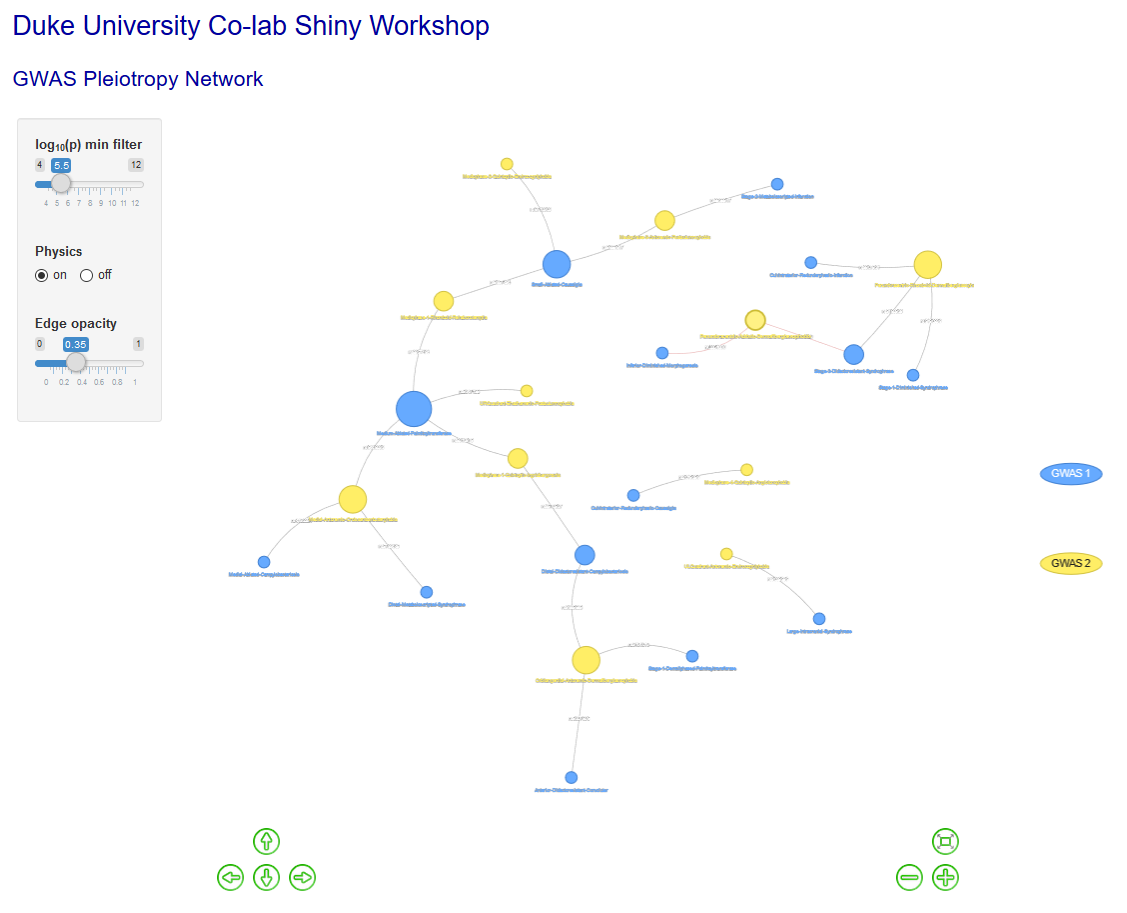
\includegraphics[width=6.5in]{visNetworkAppV1.png}}
    \centering
    \caption{\texttt{visNetwork} pleiotropy app, version 1.  Inter-GWAS phenotype as vertex, common SNP as edge.  Basic Shiny features.}
    \label{fg:visNetworkAppV1}
\end{figure}

%%%%%%%%%%%%%%%%%%%%%%%%%%%%%%%%%%%%%%%%

\subsection{\texttt{visNetwork} App Version 2, Enhanced Graph Controls}\label{sec:visNetworkV2}

Version 2 implements the following features:

\begin{itemize}[noitemsep]
    \item Phenotype or SNP vertex selection
    \item Node filtering by number of edges
    \item Subnetting graph to a selected node and all other nodes with shared edge
\end{itemize}

To execute the app locally:

\begin{itemize}[noitemsep]
    \item Download App.zip and Data.zip from\\ \url{https://github.com/tbalmat/Duke-Co-lab/tree/master/Spring-2021/Session-4-visNetwork}
    \item Expand App.zip and Data.zip in a local project directory
    \item Set the current working directory to App/V2
    \item Modify the directory reference (\texttt{setwd()} command) in App/V2/InteractivePleiotropyNetwork.r to reference the App/V2 directory on your computer
    \item Modify the directory reference (\texttt{setwd()} command) in App/V2/ui.r to reference the App/V2 directory on your computer
    \item Launch RStudio then load and execute App/V2/InteractivePleiotropyNetwork.r
\end{itemize}

Figure \ref{fg:visNetworkAppV2a} is an example screen-shot of this app with phenotype forming vertices and SNP forming edges.  App and script features for discussion include (unnn indicates line number in ui.r, snnn  indicates line number in server.r):

\begin{itemize}
  \item (u44, s94) Vertex and edge reconfiguration from phenotype/SNP to SNP/phenotype
  \item (u58, s109-110) Vertex filtering by edge count
  \item (s114-115) Vertex hover label composition
  \item Use of global variables due to events and interrupt nature of execution
  \item (s292-295) Enabling of physics stabilization
  \item (s426-429) Physics stabilization event
  \item (s305-313) Enabling of shift-click event
  \item \texttt{ignoreInit}
  \item (s498-526) Graph subnetting with shift-click (on a vertex)
  \item (u66, s529-545) Restore after subnetting
  \item (u72-74) Use of a conditional panel to create hidden reactive variables for event and interrupt control
  \item (s340-368) Hidden render instruction event.  This event coordinates graph construction and rendering based on the state of on screen controls and the current graph context.
  \item (s370-381) Hidden reactive instruction event.  Used primarily to overcome the problem of multiple, sequential function calls being ignored, except the final one.
  \item (u60, s434-442) Physics on/off event
\end{itemize}

\begin{figure}[H]
    \frame{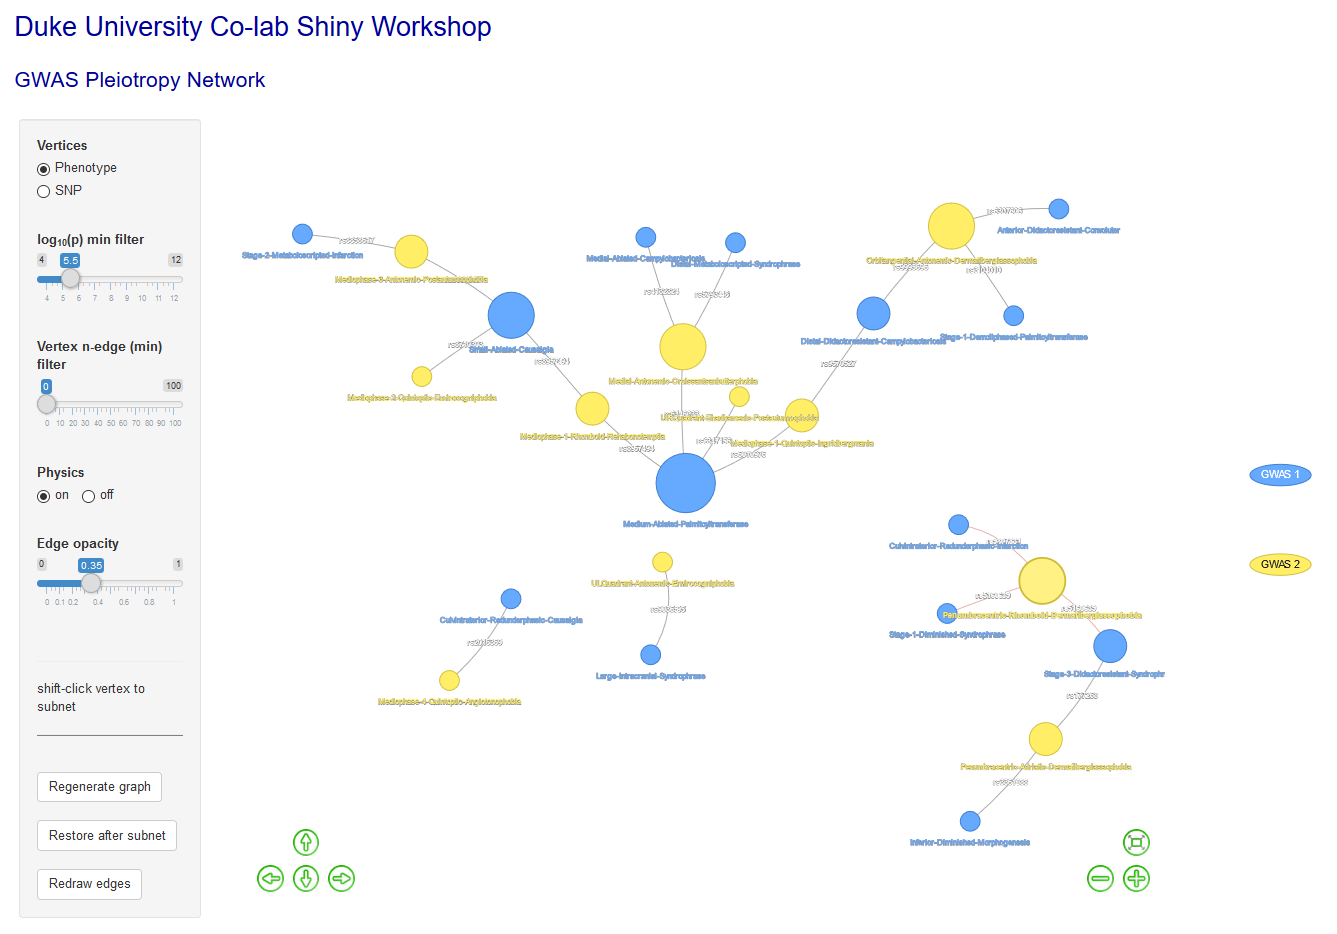
\includegraphics[width=6.5in]{visNetworkAppV2a.png}}
    \centering
    \caption{\texttt{visNetwork} pleiotropy app, version 2.  Inter-GWAS phenotype as vertex, common SNP as edge.  Additional Shiny control to filter vertices by number of edges.  Subnetting available by clicking a vertex.}
    \label{fg:visNetworkAppV2a}
\end{figure}

Figure \ref{fg:visNetworkAppV2b} is an example screen-shot with SNP forming vertices and phenotype forming edges.  The purpose of this view is to identify associations between SNPs that appear in both GWAS sets and the phenotypes that are associated with those SNPs within GWAS sets.  Vertex hover labels indicate phenotype grouping and vertex color ranges from green-blue (high proportion of GWAS 1 phenotypes in group) to green (equal proportions form both GWAS sets) to green-yellow (high proportion of GWAS 2 phenotypes).  Vertex size is proportional to the total number of phenotypes in the group.  Vertex color (continuous from blue to yellow) indicates edge SNP proportion by GWAS set.  App and script features for discussion (unnn indicates line number in ui.r, snnn  indicates line number in server.r):

\begin{itemize}
  \item (s140-158) Vertex construction
  \item (s148-158) Hover label construction
  \item (s162-185) Edge construction
  \item (s212-221) Vertex color definition
\end{itemize}

\vspace{0.25in}

\begin{figure}[H]
    \frame{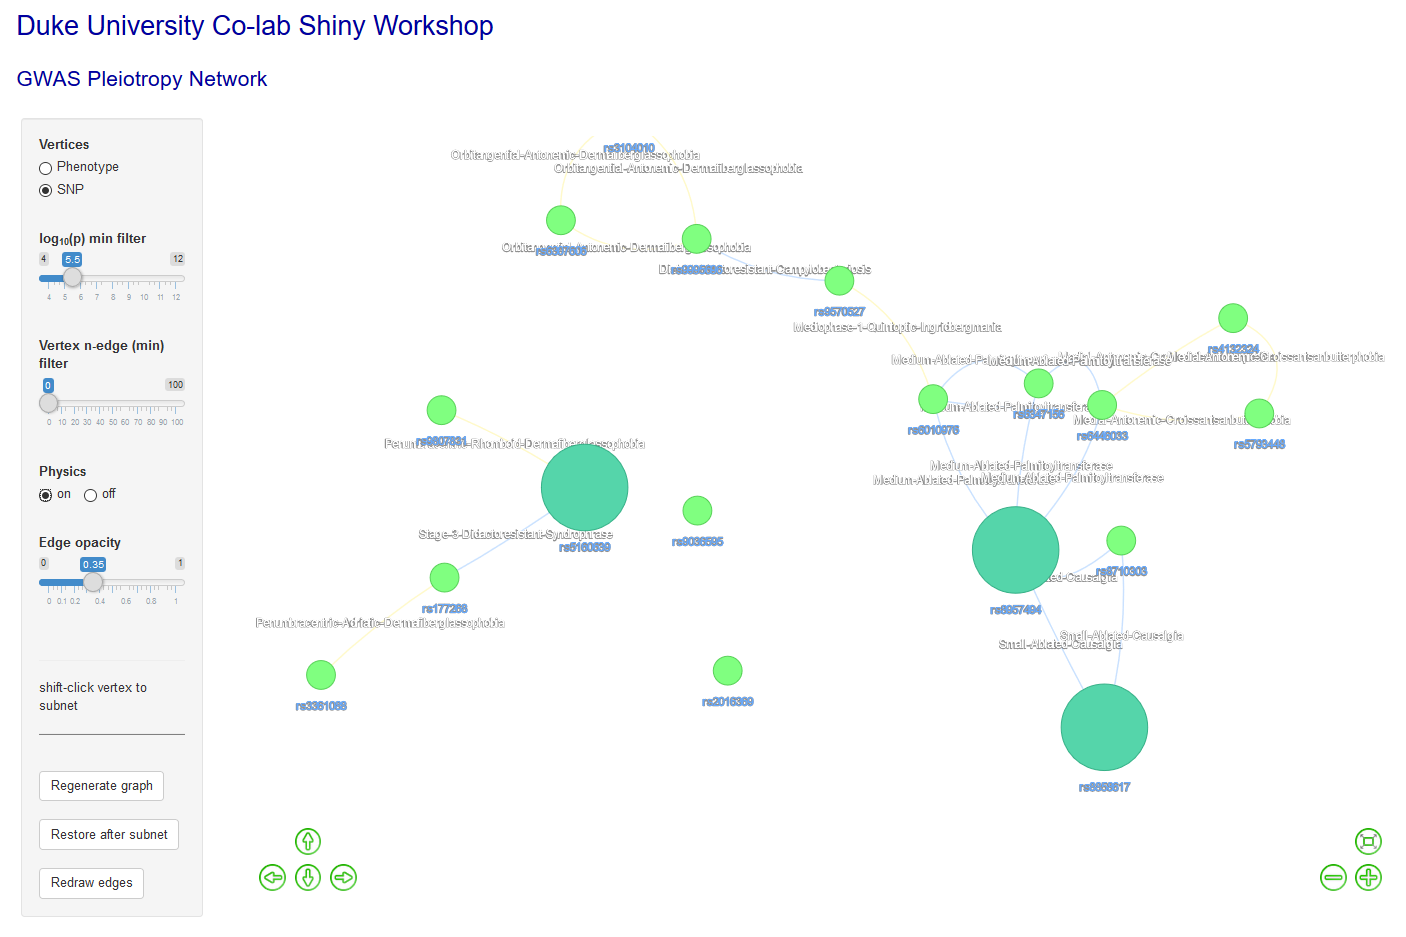
\includegraphics[width=6.5in]{visNetworkAppV2b.png}}
    \centering
    \caption{\texttt{visNetwork} pleiotropy app, version 2.  SNP as vertex, individual edge for each phenotype.  Additional Shiny control to filter vertices by number of edges.  Subnetting available by clicking a vertex.}
    \label{fg:visNetworkAppV2b}
\end{figure}

%%%%%%%%%%%%%%%%%%%%%%%%%%%%%%%

\subsection{\texttt{visNetwork} App Version 3, Additional Controls, Centrality Table}\label{sec:visNetworkV3}

Version 3 implements the following features:

\begin{itemize}[noitemsep]
    \item Node clustering (collapse of nodes having a specified number of edges into a single node)
    \item Display of a centrality table
\end{itemize}

To execute the app locally:

\begin{itemize}[noitemsep]
    \item Download App.zip and Data.zip from\\ \url{https://github.com/tbalmat/Duke-Co-lab/tree/master/Spring-2021/Session-4-visNetwork}
    \item Expand App.zip and Data.zip in a local project directory
    \item Set the current working directory to App/V3
    \item Modify the directory reference (\texttt{setwd()} command) in App/V3/InteractivePleiotropyNetwork.r to reference the App/V3 directory on your computer
    \item Modify the directory reference (\texttt{setwd()} command) in App/V3/ui.r to reference the App/V3 directory on your computer
    \item Launch RStudio then load and execute App/V1/InteractivePleiotropyNetwork.r
\end{itemize}

Figures \ref{fg:visNetworkAppV3a} and \ref{fg:visNetworkAppV3b} are example screen-shots of this app.  The primary additional feature is the centrality table.  Construction of it is accomplished in \texttt{server.r} lines 318-403.\\

\begin{figure}[H]
    \frame{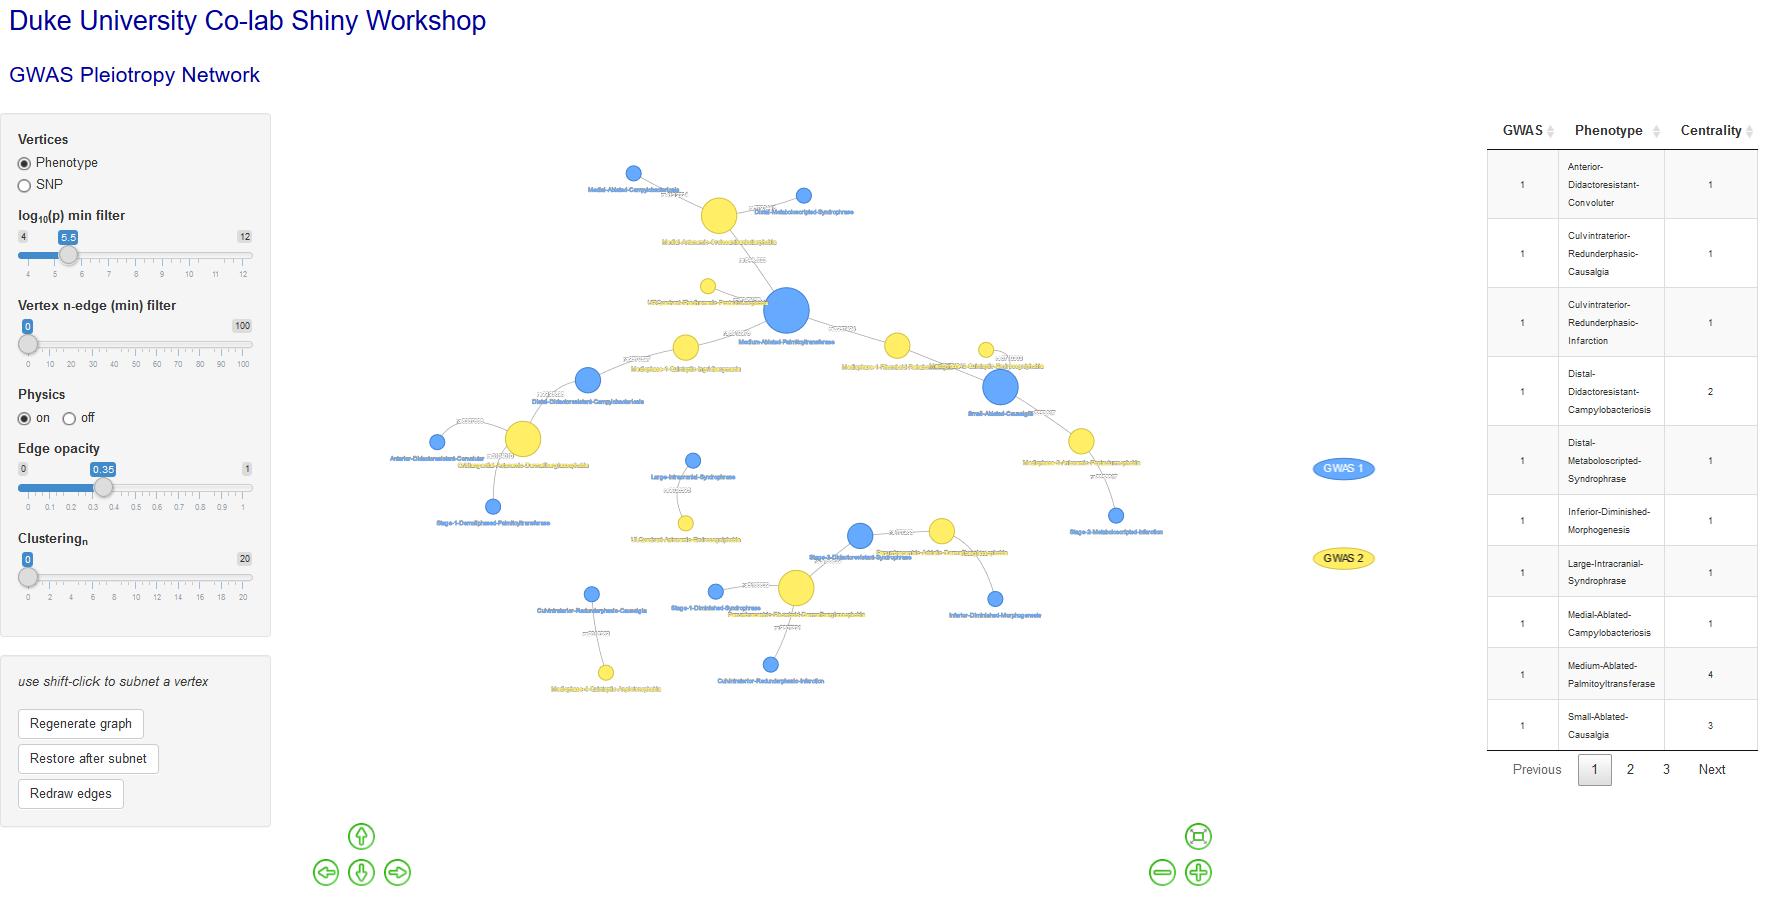
\includegraphics[width=6in]{visNetworkAppV3a.png}}
    \centering
    \caption{\texttt{visNetwork} pleiotropy app, version 3.  Inter-GWAS phenotype as vertex, common SNP as edge.  Additional Shiny control for clustering vertices.  Centrality table included.  Subnetting available by clicking a vertex.}
    \label{fg:visNetworkAppV3a}
\end{figure}

%\vspace{10pt}

\begin{figure}[H]
    \frame{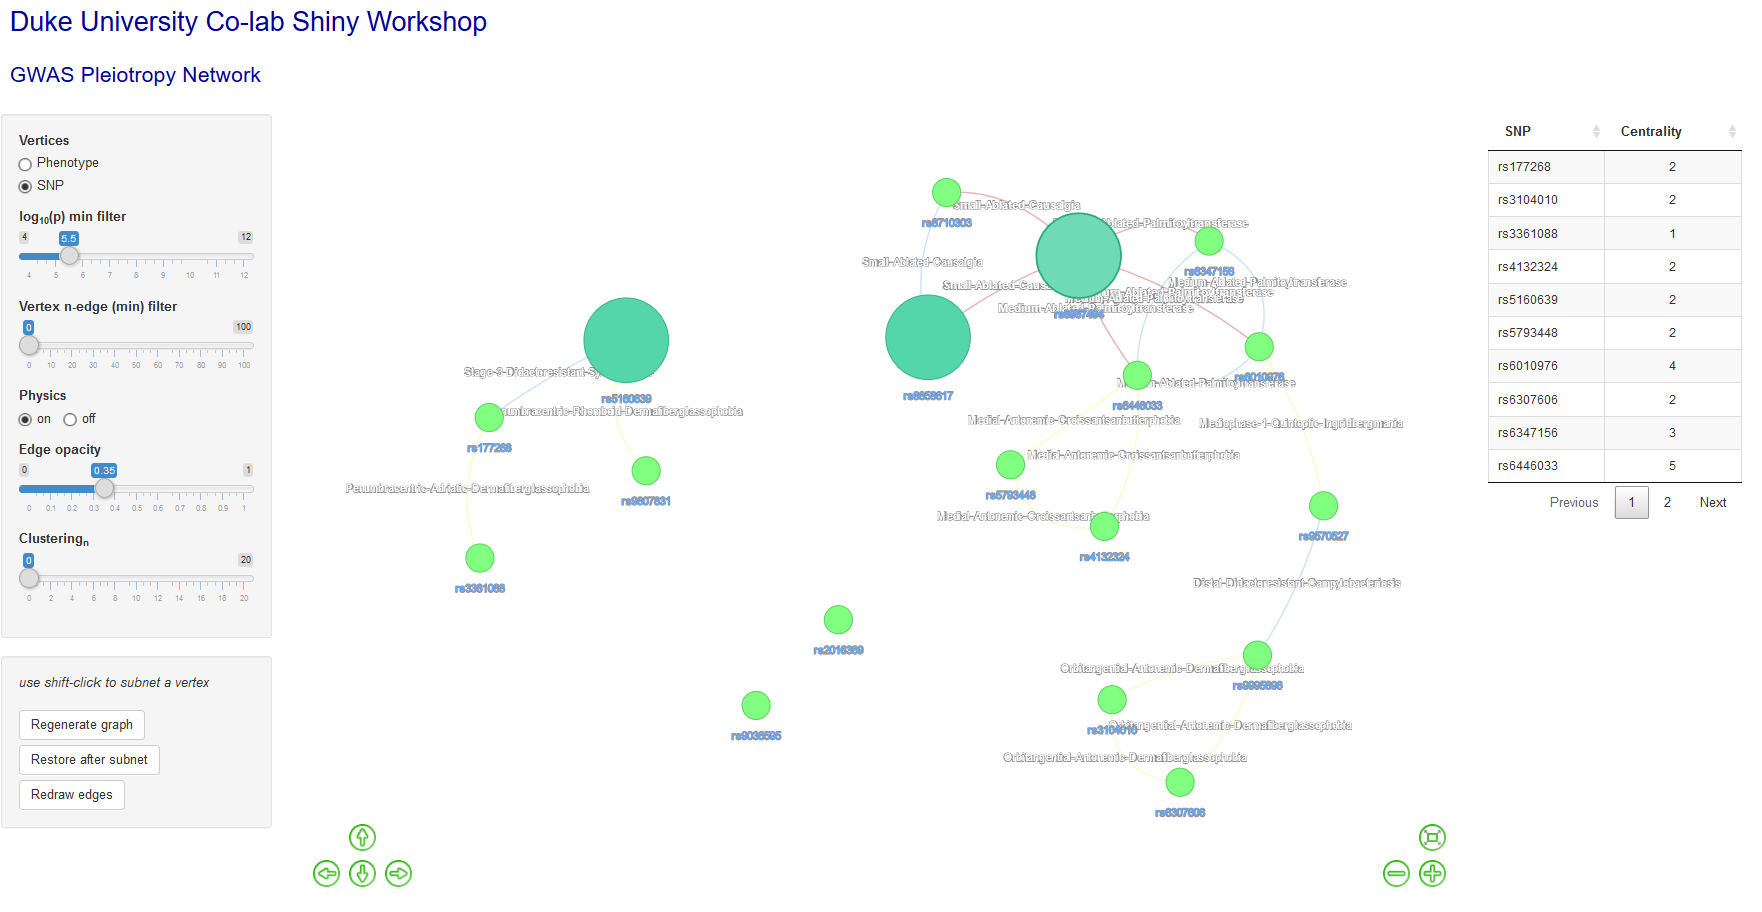
\includegraphics[width=6in]{visNetworkAppV3b.png}}
    \centering
    \caption{\texttt{visNetwork} pleiotropy app, version 3.  SNP as vertex, individual edge for each phenotype.  Additional Shiny control for clustering vertices.  Centrality table included.  Subnetting available by clicking a vertex.}
    \label{fg:visNetworkAppV3b}
\end{figure}

%%%%%%%%%%%%%%%%%%%%%%%%%%%%%%%%%%%%%%%%%%%%%%%%%%%%%%%%%%%%%%%%%%%%%%%%%%%%%%%%%%%%%%%%%%%%%%

\section{Integrating \texttt{visNetwork} with a Graph Database for Visual Data Exploration}\label{sec:UCD}

A Shiny app was developed, using \texttt{visNetwork}, for the Urea Cycle Disorder (UCD) Project in the Nursing School at Duke University.\footnote{A recent paper, currently under review, that presents important findings in UCD research, is available at \url{https://github.com/tbalmat/Duke-UCD/blob/master/Papers/ASL\_PD\_Final AE EMBO.pdf}}  \footnote{Additional information on UCD is available at \url{https://www.ncbi.nlm.nih.gov/books/NBK482363/?report=printable}} \footnote{R, Shiny, and Neo4J script sources for the Duke app are available at \url{https://github.com/tbalmat/Duke-UCD/tree/master/ShinyApp}}  Participants in the study have a specific, categorical, UCD diagnosis (UCDDx), are indicated as having or not had hyperammonemic (HA) events, and are coded for various clinically observed traits (tremors, cognitive disabilities, etc.).  Clinical observations are coded using the Semantic Nomenclature for Medicine, Clinical Terminology (SNOMED CT).\footnote{The SNOMED CT browser is available at \url{https://browser.ihtsdotools.org/}}  Researchers use the app to explore study data and visually identify associations (by unique participant frequency) between UCDDx, HA, and SNOMED CT codes.\footnote{Actually, many other variables are explored for association, but the example here is limited to UCDDx, HA, and SNOMED CT code} \footnote{For an overview of using the app along with some example graphs, see \url{https://github.com/tbalmat/Duke-UCD/blob/master/ShinyApp/Overview/UCDAppOverview01/UCDAppOverview01.pdf}}  An interesting feature of the project is its database.  Instead of using SQL or an unstructured data format, all participant, diagnosis, SNOMED CT, and prescribed drug data along with their relational associations are represented in a Neo4J graph database.\footnote{\url{https://neo4j.com/}} \footnote{For a discussion of encoding SNOMED CT concept paths in a Neo4J database, see \url{https://www.sciencedirect.com/science/article/pii/S1532046415001847}}  Important features of the app are the ability to select nodes for filtering or expansion.  Filtering limits nodes to a select group, while expansion explores the subnet of selected nodes, allowing step-wise exploration, in increasing detail, of participant and medical diagnosis relationships as the researcher encounters them.  The following demonstrates construction of a graph and use of node selection, filtering, and expansion operations.\\

\subsection{SNOMED CT Concept Selection}

Although multiple concepts can be selected, the example is limited to one, \textit{Involuntary movement}.  All immediate members, in the SNOMED CT hierarchy, of \textit{Involuntary movement} will be displayed on the graph.  Later, we will expand the \textit{Tremor} sub-concept of \textit{Involuntary movement} to explore this important clinical diagnosis.  \textit{Involuntary movement} appears in the SNOMED CT hierarchy under \textit{Clinical finding}, \textit{Clinical history and observation findings}, \textit{Finding of movement}.  Figure \ref{fg:UCD01} Shows the concept selector (under ``1. Explore concepts").  The selection hierarchy list follows that of the SNOMED CT browser.  Once a concept is selected (under ``2. Select concepts") the UCD Neo4J graph database is queried (``3. query").

\begin{figure}[H]
    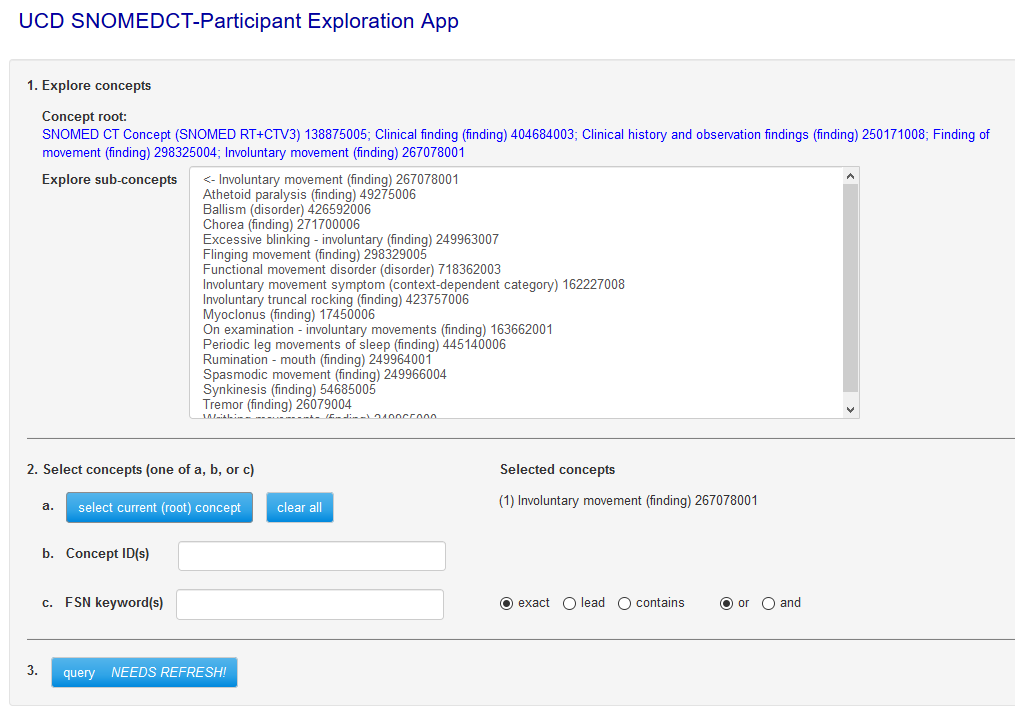
\includegraphics[width=6in]{UCD01.png}
    \centering
    \caption{Duke University UCD app.  Selection of SNOMED CT \textit{Involuntary movement} concept.}
    \label{fg:UCD01}
\end{figure}

\subsection{Define Node and Edge Variables}

Figure \ref{fg:UCD02} shows the node and edge variable selection check boxes.  Here, we have selected UCDDx, HA, and SNOMED CT concept as nodes, with edges between UCDDx and HA and between UCDDx and concept.  Group-HA has also been specified causing the various HA database values to be classified as either HA or not HA.  Figure \ref{fg:UCD03} shows the resulting graph.  Nodes are colored by variable and sized by number of unique participants assigned to the variable level associated with a node.  Edges are sized according to the number of unique participants assigned both variable levels of nodes that are joined by a particular edge.  Note that free-form selection of node and edge variables allows construction of a wide variety of graphs.  Variable configuration can be changed after graph subsetting and node expansion to allow for exploration of further relationships as study data are visually probed in increasing detail.\\

\begin{figure}[H]
    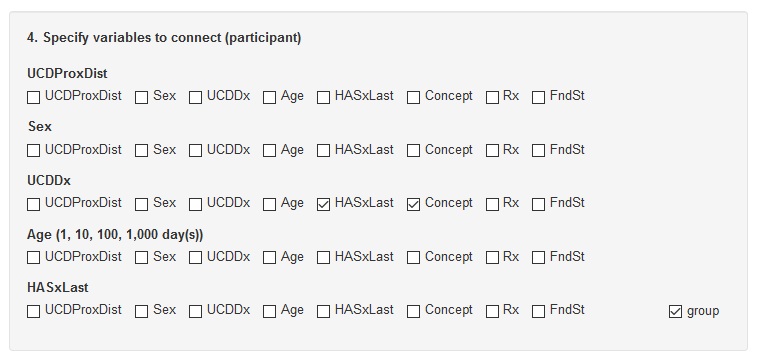
\includegraphics[width=4in]{UCD02.png}
    \centering
    \caption{Duke University UCD app.  Node and edge variable selection.}
    \label{fg:UCD02}
\end{figure}

\begin{figure}[H]
    \frame{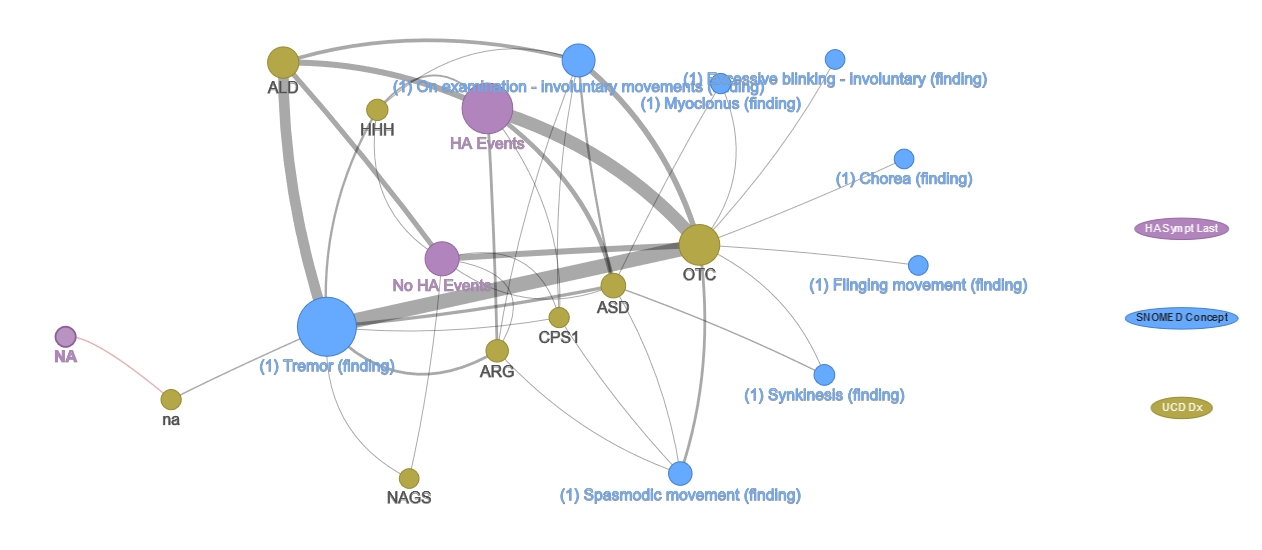
\includegraphics[width=6in]{UCD03.png}}
    \centering
    \caption{Duke University UCD app.  Graph of UCDDx, HA, and \textit{Involuntary movement} SNOMED CT concept.}
    \label{fg:UCD03}
\end{figure}

\subsection{Subset Graph to Isolate Variable Levels of Interest}

Often, a researcher specializes in particular levels, or varieties, of variables within a system and would like to limit a graph to levels of interest.  Figure \ref{fg:UCD04} shows selection of desired nodes (depressing the shift key simultaneous with clicking the left mouse, or shift-click, selects and highlights nodes).  The ``subnet" button (figure \ref{fg:UCD05}, under ``7. Explore") executes node subsetting and graph regeneration.  Figure \ref{fg:UCD06} shows the resulting graph.  Nodes appearing without edges are for reference and indicate variable levels of nodes that shared an edge to a UCDDx node in the complete graph, but not of levels ALD or ASD.\\

\begin{figure}[H]
    \frame{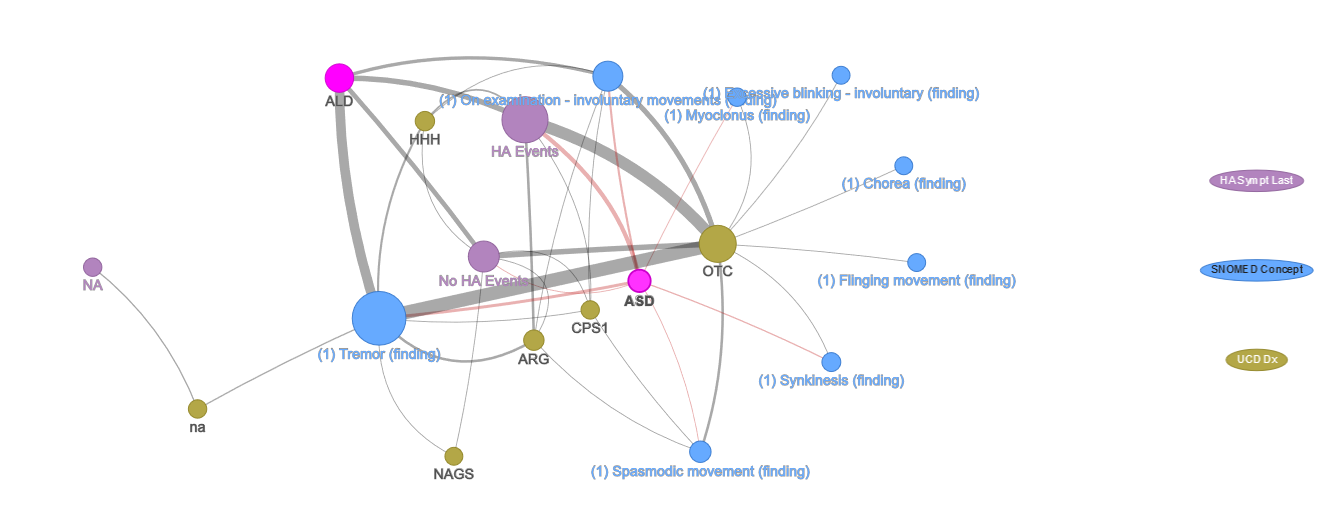
\includegraphics[width=6in]{UCD04.png}}
    \centering
    \caption{Duke University UCD app.  Selection of UCDDx levels ALD and ASD for graph subsetting.}
    \label{fg:UCD04}
\end{figure}

\begin{figure}[H]
    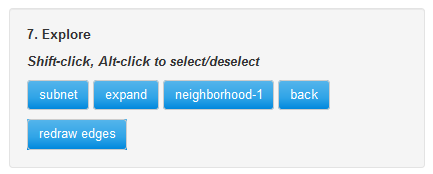
\includegraphics[width=3in]{UCD05.png}
    \centering
    \caption{Duke University UCD app.  The subnet button used to subset graph to selected nodes.}
    \label{fg:UCD05}
\end{figure}

\begin{figure}[H]
    \frame{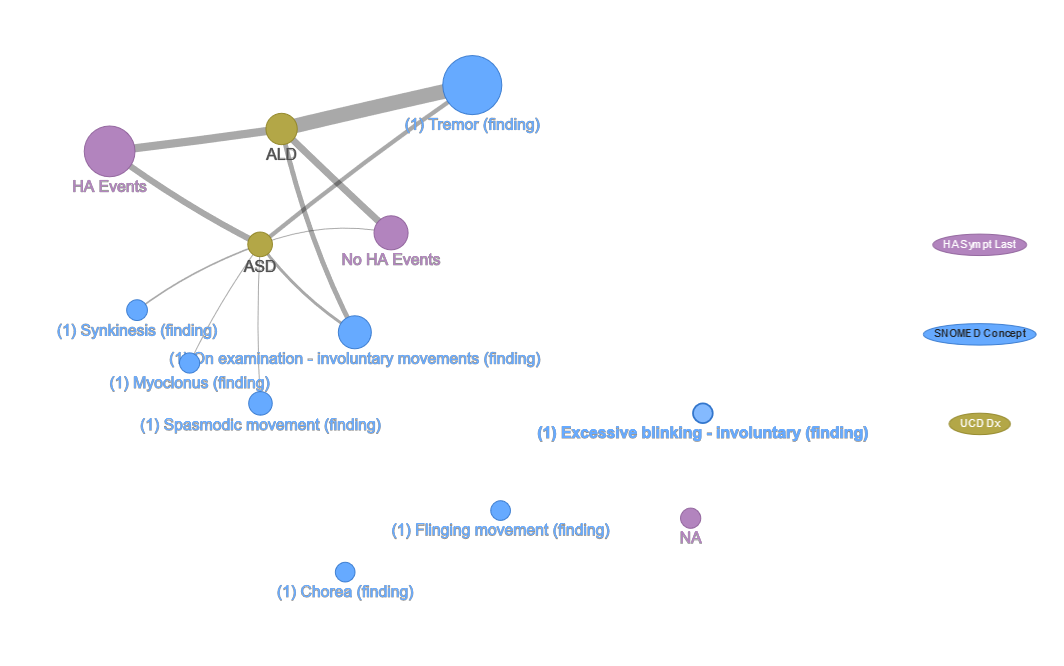
\includegraphics[width=6in]{UCD06.png}}
    \centering
    \caption{Duke University UCD app.  Graph resulting from UCDDx ALD and ASD selection and subsetting.}
    \label{fg:UCD06}
\end{figure}

\subsection{Expansion of a Select SNOMED CT Concept Node}

In the SNOMED CT hierarchy path explored here, the concept \textit{Tremor} has multiple immediate concept members.  To expand the \textit{Tremor} node and present a graph of UCDDx (limited to ALD and ASD, since subsetting remains), HA, and \textit{Tremor} concept members, we select the \textit{Tremor} node (shift-click, figure \ref{fg:UCD07}) and click the expand button (figure \ref{fg:UCD05}).  Note the label (``n=72") that appears when hovering over a node (figure \ref{fg:UCD07}).  Here, the label indicates that 72 unique participants are assigned a SNOMED CT concept that is an immediate member of \textit{Tremor} (when \textit{Tremor} is selected at this place in the SNOMED CT hierarchy - it may appear in other hierarchical positions with a different number of unique participants assigned).  Figure \ref{fg:UCD08} shows the graph produced by expanding \textit{Tremor}.  Hover labels in figures \ref{fg:UCD09} through \ref{fg:UCD11} indicate 18 unique participants assigned \textit{Intention tremor}, 17 unique participants assigned UCD diagnosis of ALD, and 12 unique participants assigned both \textit{Intention tremor} and ALD, since corresponding nodes share an edge.  Note that \textit{Intention tremor} is associated with (shares an edge) with UCD diagnosis ALD, but not with ASD.  This may be an important finding, or it may confirm researcher intuition based on clinical experience.

\begin{figure}[H]
    \frame{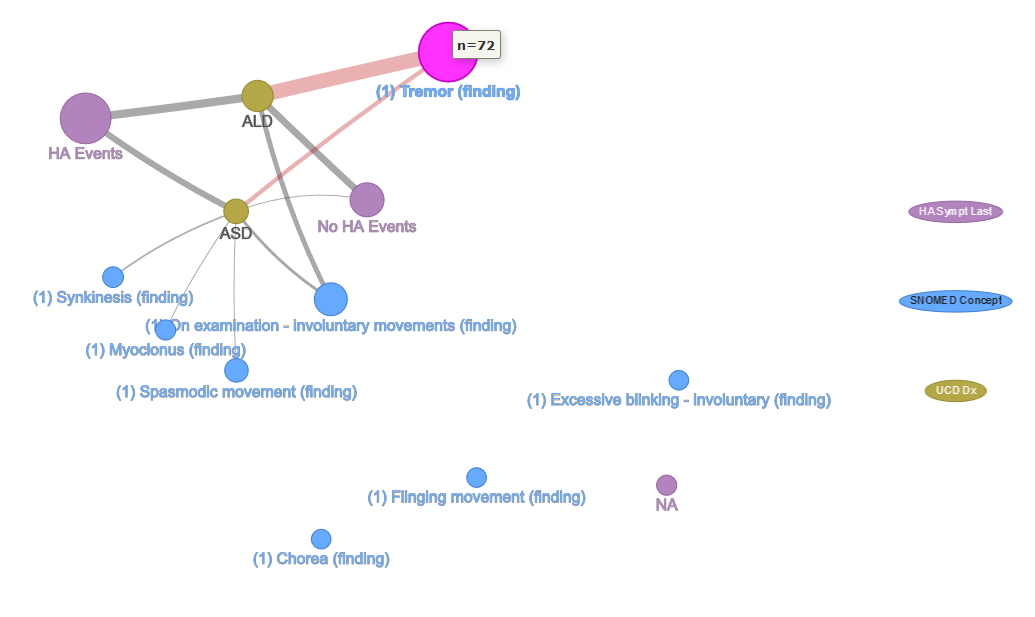
\includegraphics[width=6in]{UCD07.png}}
    \centering
    \caption{Duke University UCD app.  Selection of \textit{Tremor} concept node for expansion.}
    \label{fg:UCD07}
\end{figure}

\begin{figure}[H]
    \frame{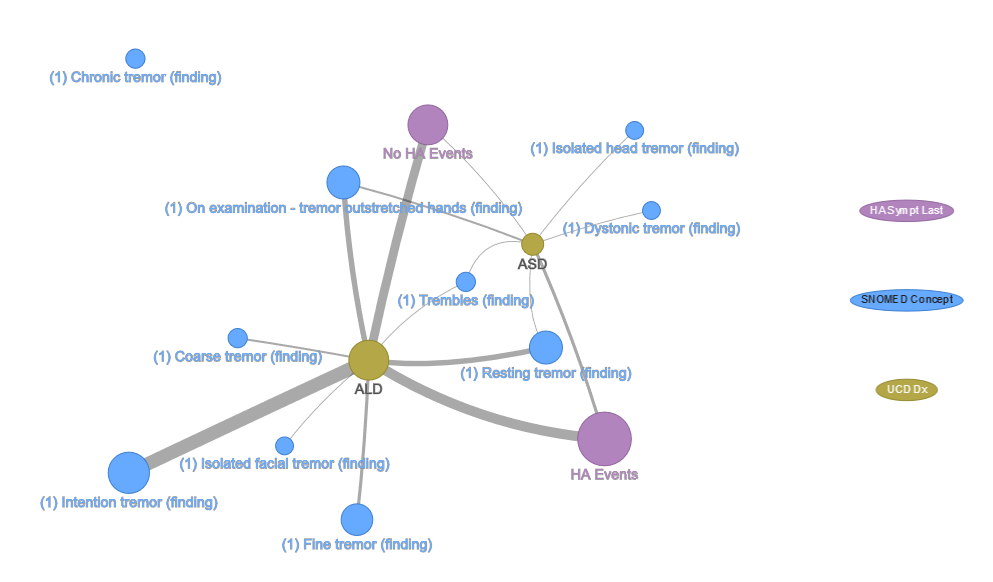
\includegraphics[width=6in]{UCD08.png}}
    \centering
    \caption{Duke University UCD app.  Graph resulting from \textit{Tremor} concept node expansion.}
    \label{fg:UCD08}
\end{figure}

\begin{figure}[H]
    \frame{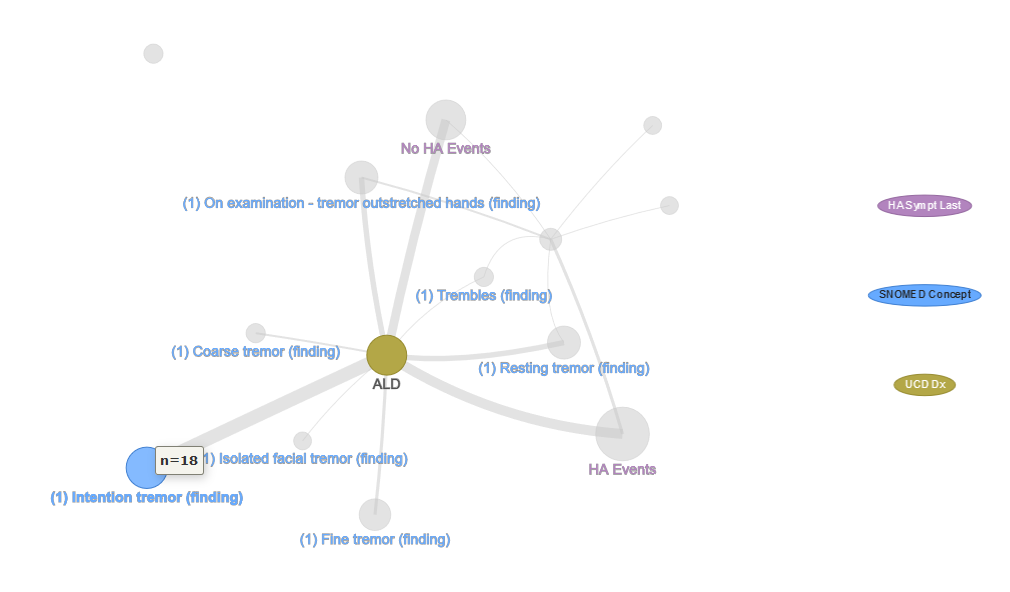
\includegraphics[width=6in]{UCD09.png}}
    \centering
    \caption{Duke University UCD app.  Hover label indicating 18 unique participants assigned \textit{Intention tremor} concept.}
    \label{fg:UCD09}
\end{figure}

\begin{figure}[H]
    \frame{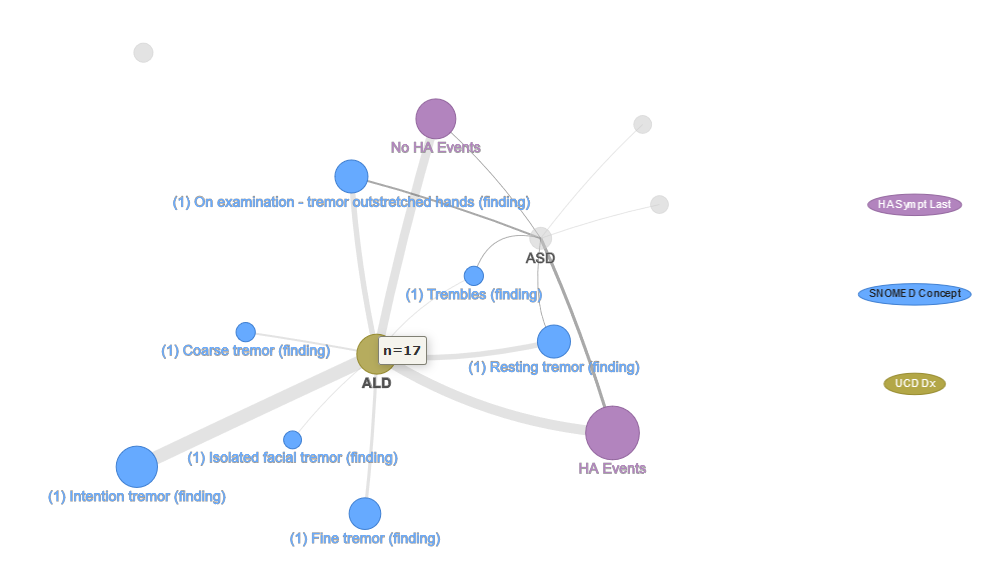
\includegraphics[width=6in]{UCD10.png}}
    \centering
    \caption{Duke University UCD app.  Hover label indicating 17 unique participants assigned UCDDx level of ALD.}
    \label{fg:UCD10}
\end{figure}

\begin{figure}[H]
    \frame{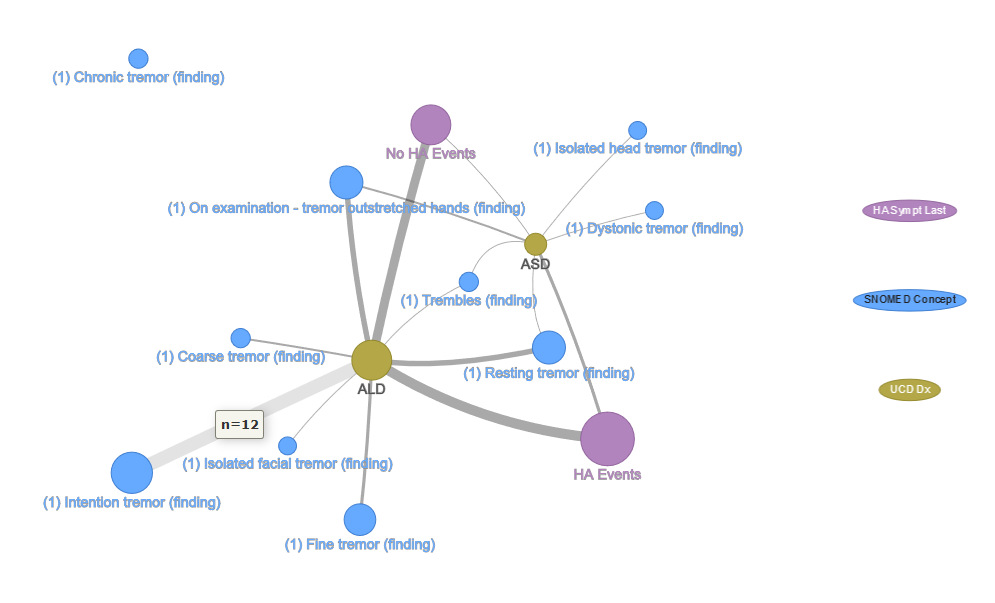
\includegraphics[width=6in]{UCD11.png}}
    \centering
    \caption{Duke University UCD app.  Hover label indicating 12 unique participants assigned (sharing an edge) both \textit{Intention tremor} and UCDDx level of ALD.}
    \label{fg:UCD11}
\end{figure}

\subsection{Radial Graph}

An alternative to the free-form graphs presented so far is a radial presentation.  Figure \ref{fg:UCD12} shows selection of ``radial" on the alternative geometry configurator and figure \ref{fg:UCD13} shows the resulting graph (nodes and edges are identical to those in figure \ref{fg:UCD08}).  Note that concept and UCDDx imbalance are indicated by concepts with a single UCDDx edge, which is, perhaps, more visible in the radial than in the free-form graph.\\

\begin{figure}[H]
    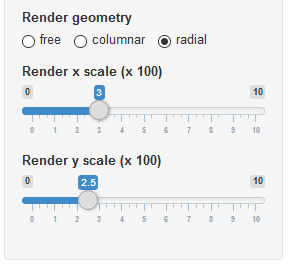
\includegraphics[width=2in]{UCD12.png}
    \centering
    \caption{Duke University UCD app.  Radial graph layout specification.}
    \label{fg:UCD12}
\end{figure}

\begin{figure}[H]
    \frame{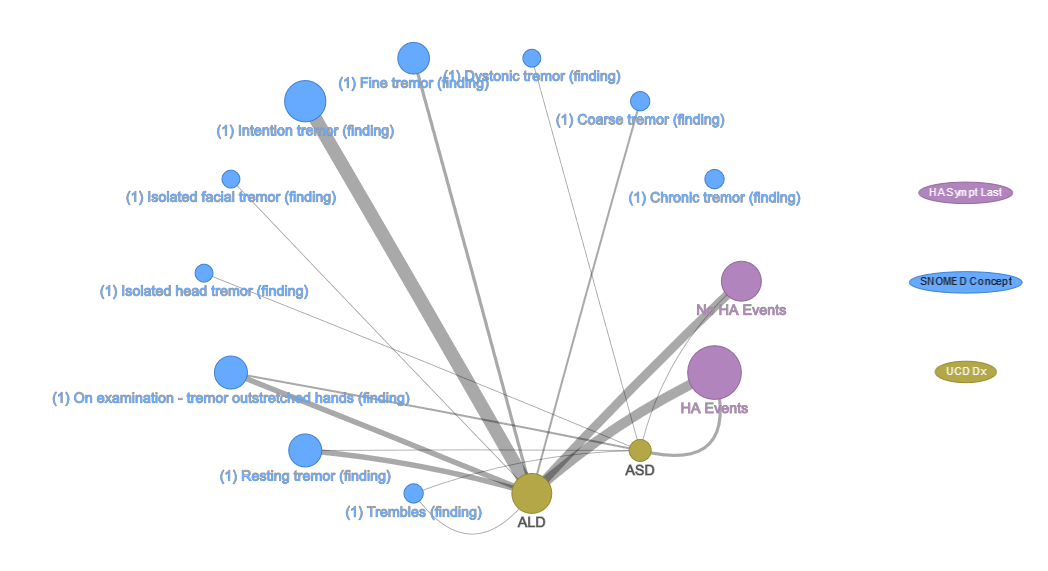
\includegraphics[width=6in]{UCD13.png}}
    \centering
    \caption{Duke University UCD app.  Radial graph layout.}
    \label{fg:UCD13}
\end{figure}

\subsection{Interactions}

Graphs presented so far assume that relationships between levels of two variables hold regardless of the level of a third variable.  However, given our data, it may be the case that relationships between, say UCDDx and HA, depend on the level of SNOMED CT concept.  For instance, if UCDDx of ALD is associated with concept \textit{Trembles} only when HA is positive, we want our graph to indicate this interaction with corresponding edges.  Figure \ref{fg:UCD14} shows interaction controls.  Figures \ref{fg:UCD15} and \ref{fg:UCD16} show the resulting graph in free-form and columnar (bipartite) formats, respectively.

\vspace{0.25in} 

\begin{figure}[H]
    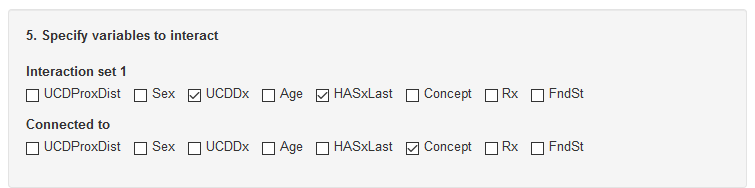
\includegraphics[width=4.5in]{UCD14.png}
    \centering
    \caption{Duke University UCD app.  Specifying interactions.}
    \label{fg:UCD14}
\end{figure}

\vspace{0.25in}

\begin{figure}[H]
    \frame{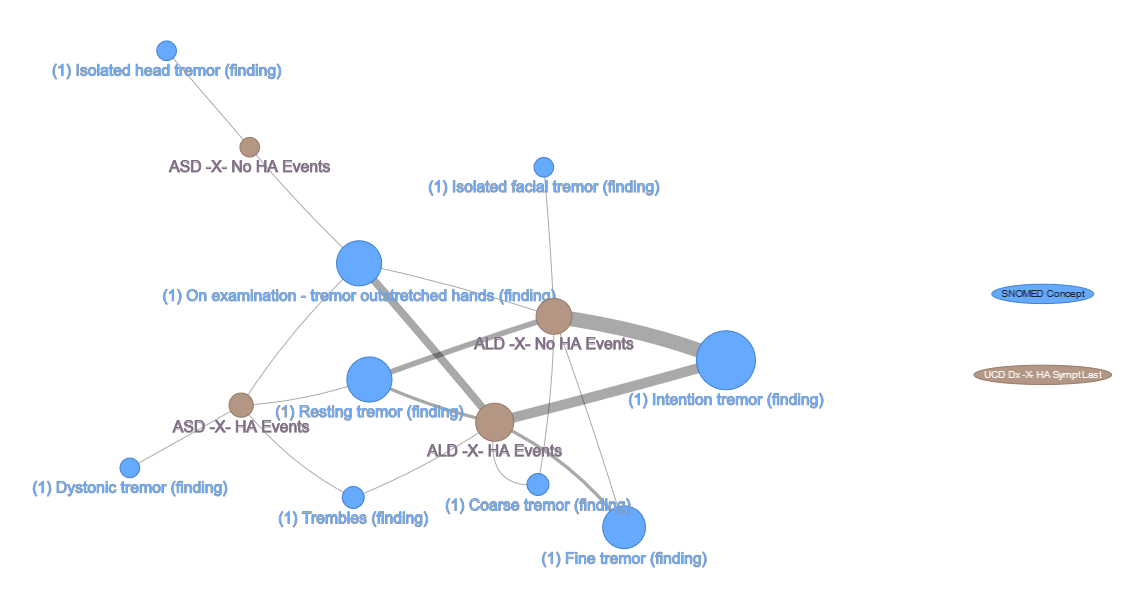
\includegraphics[width=6in]{UCD15.png}}
    \centering
    \caption{Duke University UCD app.  Interaction graph, free-form.}
    \label{fg:UCD15}
\end{figure}

\begin{figure}[H]
    \frame{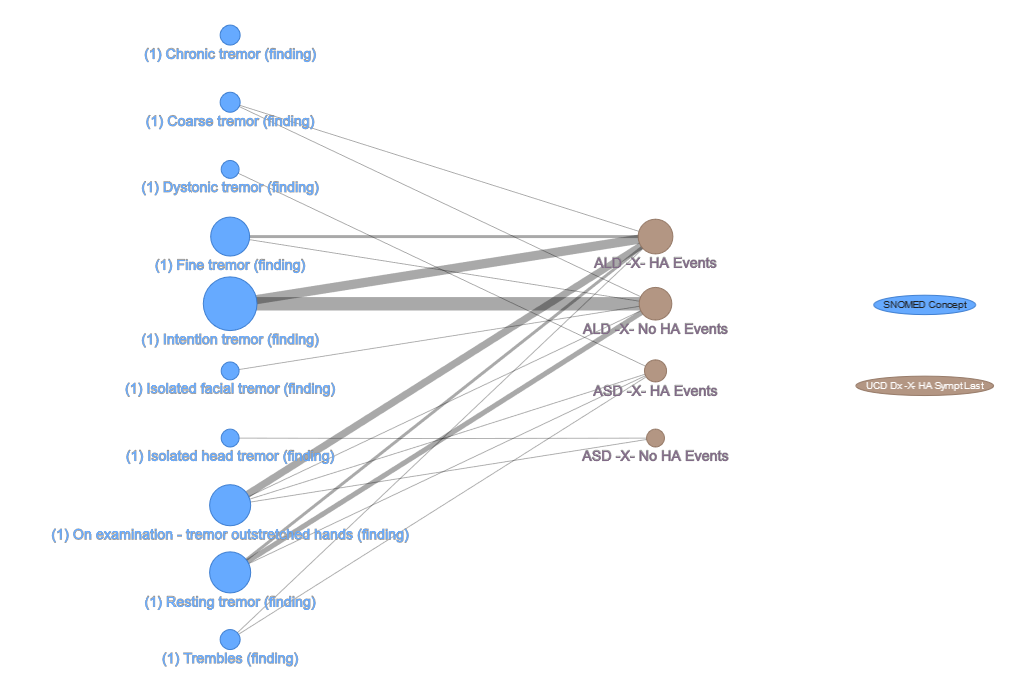
\includegraphics[width=6in]{UCD16.png}}
    \centering
    \caption{Duke University UCD app.  Interaction graph, bipartite.}
    \label{fg:UCD16}
\end{figure}

%%%%%%%%%%%%%%%%%%%%%%%%%%%%%%%%%%%%%%%%%%%%%%%%%%%%%%%%%%%%%%%%%%%%%%%%%%%%%%%%%%%%%%%%%%%%%%

\section{Alternative Visualizations}\label{sec:altvis}

Script location:  \url{https://github.com/tbalmat/Duke-UCD/blob/master/ShinyApp/AlternativeVisualization/UCDEdgeBundle.r}\\

The following instructions use the \texttt{ggraph()} function of the \texttt{ggraph} package to produce various hierarchical and edge bundled graphs that may serve as alternatives to network graphs.\footnote{For more information on the \texttt{ggraph} package, see \url{https://ggraph.data-imaginist.com/reference/index.html}}  Each set of instructions is executed after querying the UCD graph database mentioned in section \ref{sec:UCD}.  Variables in the queried result set are participant, the interaction between UCD diagnosis and hyperammonemia classification, SNOMED concept, and prescribed medication.

\subsection{Create Hierarchy, Vertices, and Initial Graph}

\small
\begin{verbatim}
                #######################################################################################
                # Create hierarchy
                # The dendrogram has an origin for groups, an origin for each group, and leaves (try
                # ggraph with circular=F)
                # From and to, here, instruct from which graph origin a line originates and where it
                # terminates
                # The groups originate at the origin and termnate at a group
                # The leaves originate at a group and terminate in a leaf (the unique label within the
                # data for a group)
                #######################################################################################
                
                h <- rbind(data.frame("from"="origin", "to"="origin",
                                      "n"=length(unique(y[,"participantID"]))),
                           data.frame("from"="origin", "to"=v,
                                      "n"=length(unique(y[,"participantID"]))),
                do.call(rbind, lapply(v,
                  function(v)
                    setNames(aggregate(1:nrow(y), by=list(rep(v, nrow(y)), y[,v]),
                               function(k) length(unique(y[k,"participantID"]))),
                             c("from", "to", "n")))))
                
                #######################################################################################
                # Create vertices
                #######################################################################################
                
                vertex <- setNames(h[,c("to", "from", "n")], c("name", "v", "n"))
                
                #######################################################################################
                # Create igraph hierarchical dendrogram object
                #######################################################################################
                
                g <- graph_from_data_frame(h, vertices=vertex)
\end{verbatim}
\normalsize

\subsection{Hierarchical Dendrogram Edges Indication Pathways Between Node Types}

Script:
\small
\begin{verbatim}
                # Review plot and group origins
                ggraph(g, layout='dendrogram', circular=F) + 
                  geom_edge_diagonal() +
                  theme_void()
\end{verbatim}
\normalsize

Result:

\begin{figure}[H]
    \frame{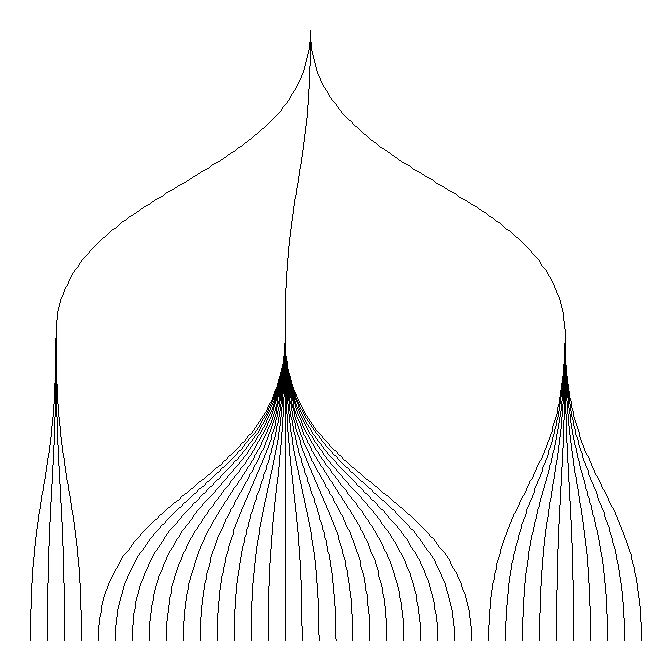
\includegraphics[width=4.5in]{Dendrogram1.png}}
    \centering
    \caption{Hierarchical UCD dendrogram showing pathways between node types}
    \label{fg:dend1}
\end{figure}

\subsection{Hierarchical Dendrogram Edges and Nodes}

Script:
\small
\begin{verbatim}
                # Add points
                ggraph(g, layout='dendrogram', circular=F) +
                  # x, y coordinates are generated by ggraph() (use str(ggraph(...)) to review elements)
                  # n is taken from the vertex data frame used to construct g
                  geom_node_point(aes(x=x, y=y, size=n)) +
                  geom_edge_diagonal() +
                  theme_void()
\end{verbatim}
\normalsize

Result:

\begin{figure}[H]
    \frame{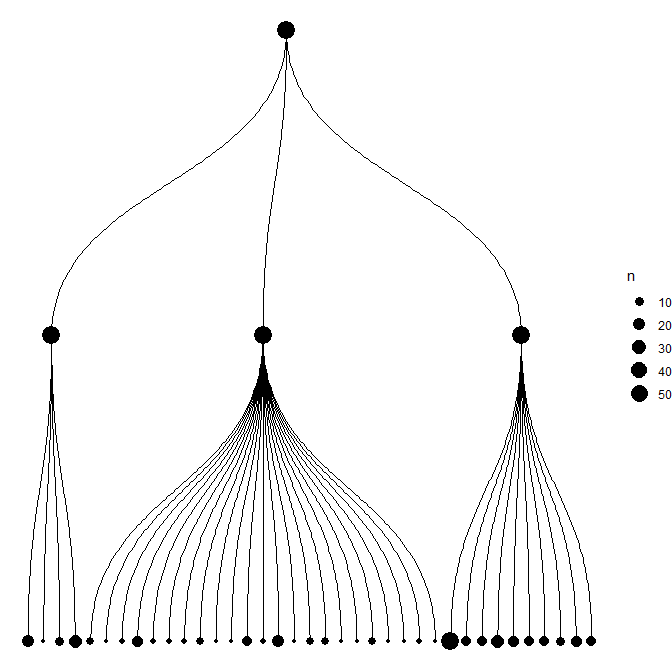
\includegraphics[width=4.5in]{Dendrogram2.png}}
    \centering
    \caption{Hierarchical UCD dendrogram with edges and nodes}
    \label{fg:dend2}
\end{figure}

\subsection{Hierarchical Dendrogram Edges Indicing Unique Participant Frequency by Node Type}

Script:
\small
\begin{verbatim}
                # Add points
                ggraph(g, layout='dendrogram', circular=F) +
                  # x, y coordinates are generated by ggraph() (use str(ggraph(...)) to review elements)
                  # n is taken from the vertex data frame used to construct g
                  geom_node_point(aes(x=x, y=y, size=n)) +
                  geom_edge_diagonal() +
                  theme_void()
                
                # Add labels
                ggraph(g, layout='dendrogram', circular=F) +
                  # Coordinates:
                  # Plot extents are (0,0) to (n_leaves-1,n_levels-1), where n_levels is the number of levels in the
                  # hierarchy (one for origin to origin, one for the groups with from="origin," and one for leaves)
                  # leaves are placed at x=0..n_leaves-1, y=0
                  # x, y coordinates are generated by ggraph() (use str(ggraph(...)) to review elements)
                  # v and n are taken from the vertex data frame used to construct g
                  geom_node_point(aes(x=x, y=y, size=n,
                    color=ifelse(v!="origin", v, ifelse(name!="origin", name, "Participants")))) +
                  geom_node_text(aes(x=ifelse(v!="origin", x, x+1),
                    y=ifelse(v!="origin", y-0.2, y),
                    label=ifelse(name!="origin", name, "Participant"), #paste("(", x, ",", y, ")", sep=""),
                    color=ifelse(v!="origin", v, ifelse(name!="origin", name, "Participants")),
                    angle=ifelse(v!="origin", 90, 0),
                    vjust=0.5,
                    hjust=ifelse(v!="origin", 1, 0),
                    # Note that node and text sizes are from disjoint spaces, but ggplot does not
                    # support multiple scale_size functions
                    # Therefore, scale text the range of point sizes, which are based on participant
                    # counts
                    size=ifelse(v!="origin", 10, ifelse(name!="origin", 20, 30)))) +
                  scale_color_manual(values=setNames(c("black",
                    rgb(matrix(col2rgb("#FFEE66"), nrow=1)/390),
                    rgb(matrix(col2rgb("#66AAFF"), nrow=1)/300),
                    rgb(matrix(col2rgb("#88AAAA"), nrow=1)/280)), c("Participants", v)),
                    guide=F) +
                  #scale_size_manual(values=c("t1"=3, "t2"=4, "t3"=5), guide=F) +
                  geom_edge_diagonal() +
                  expand_limits(x=c(NA, length(which(h[,"from"]!="origin"))+5), y=c(-2.5, NA)) +
                  theme_void() + theme(plot.margin=margin(0.25, 0.25, 0.25, 0.25, "in"))
\end{verbatim}
\normalsize

Result (n indicates unique participant frequency):\\

\begin{figure}[H]
    \frame{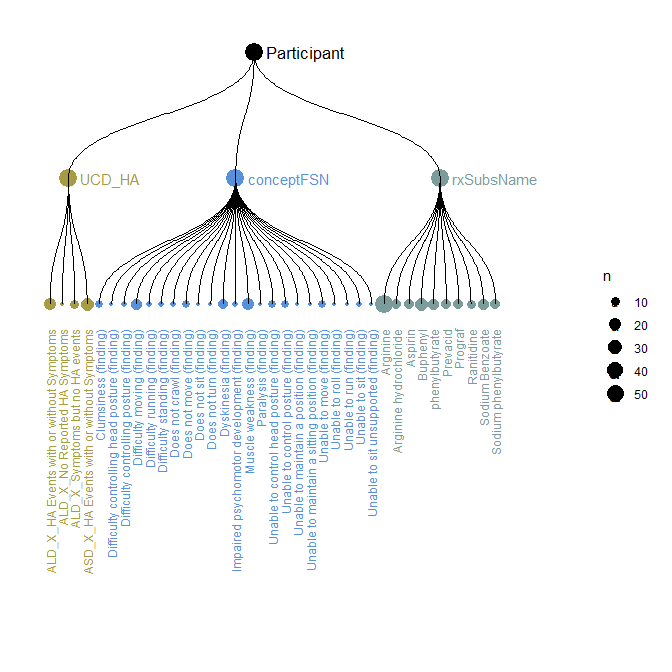
\includegraphics[width=4.5in]{Dendrogram3.png}}
    \centering
    \caption{Hierarchical UCD dendrogram with nodes sized to indicate unique participant frequency}
    \label{fg:dend3}
\end{figure}

\subsection{Radial Edge Bundled Graph (points and edges)}

Script:
\small
\begin{verbatim}
                # Include points (nodes)
                ggraph(g, layout='dendrogram', circular=T) +
                  # x, y coordinates are generated by ggraph() (use str(ggraph(...)) to review elements)
                  # Filter=leaf omits points for graph and group origins
                  geom_node_point(aes(x=x*1.05, y=y*1.05, filter=leaf)) +
                  # from and to are taken from the edge data frame
                  geom_conn_bundle(data=get_con(from=edge[,"from"], to=edge[,"to"]),
                  color="blue", alpha=0.1, tension=0.75) +
                  theme_void()
\end{verbatim}
\normalsize

Result:

\begin{figure}[H]
    \frame{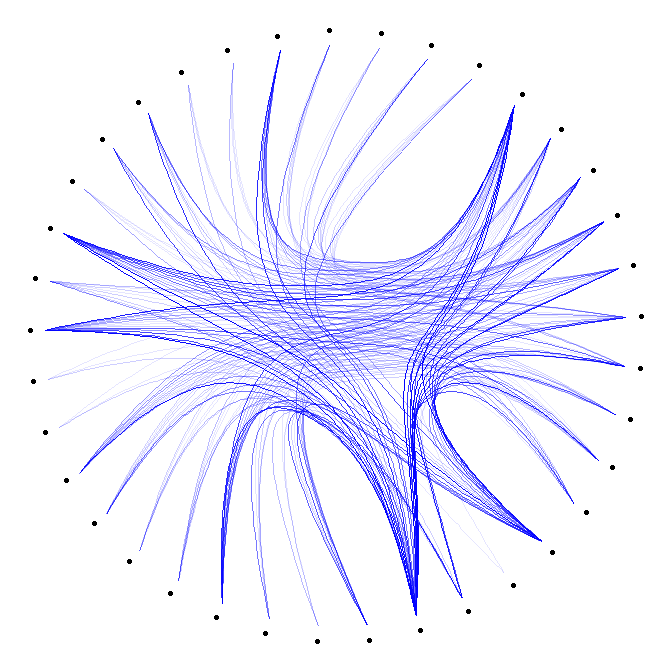
\includegraphics[width=4.5in]{EdgeBundle1.png}}
    \centering
    \caption{UCD radial edge bundled graph, nodes and edges only}
    \label{fg:edgebund1}
\end{figure}

\subsection{Radial Edge Bundled Graph with Edges, Nodes Sized for n, and Node Labels}

Script:
\small
\begin{verbatim}
                # Draw points, labels, and edges, sized and colored
                xyfactor <- 3
                glim <- c(-10, 10)
                tsize <- 3.5
                ecolor <- setNames(c(rgb(matrix((col2rgb("#FFEE66")+col2rgb("#66AAFF"))/2, nrow=1)/300),
                rgb(matrix((col2rgb("#FFEE66")+col2rgb("#88AAAA"))/2, nrow=1)/300),
                rgb(matrix((col2rgb("#66AAFF")+col2rgb("#88AAAA"))/2, nrow=1)/300)),
                apply(t(combn(1:3, 2)), 1, function(j) paste(v[j[1]], "_", v[j[2]], sep="")))
               
                ggraph(g, layout='dendrogram', circular=T) +
                  # Draw arcs first, so that points overlay ends
                  # x, y coordinates are generated by ggraph() (use str(ggraph(...)) to review elements)
                  # from and to are taken from the edge data frame
                  geom_conn_bundle(data=get_con(from=edge[,"from"], to=edge[,"to"], v12=edge[,"v12"]),
                    aes(x=x*xyfactor, y=y*xyfactor, color=v12), edge_width=0.35, alpha=0.1, tension=0.75) +
                  scale_edge_color_manual(values=ecolor) +
                  # v and n are taken from the vertex data frame used to construct g
                  geom_node_point(aes(filter=leaf, x=x*xyfactor, y=y*xyfactor, size=n, color=v), alpha=0.8) +
                  scale_size_continuous(range=c(3, 10)) +
                  geom_node_text(aes(x=xyfactor*1.2*x, y=xyfactor*1.2*y, filter=leaf, label=name, color=v,
                    angle=ifelse((node_angle(x, y)+270)%%360 > 180, 0, 180)+node_angle(x, y),
                    vjust=ifelse((node_angle(x, y)+270)%%360 > 180, 0.25, 0.5)), size=tsize, hjust="outward") +
                  scale_color_manual(values=setNames(c(rgb(matrix(col2rgb("#FFEE66"), nrow=1)/390),
                    rgb(matrix(col2rgb("#66AAFF"), nrow=1)/300),
                    rgb(matrix(col2rgb("#88AAAA"), nrow=1)/280)), v)) +
                theme_void() +
                theme(legend.position="none") +
                expand_limits(x=glim, y=glim)
\end{verbatim}
\normalsize

Result:

\begin{figure}[H]
    \frame{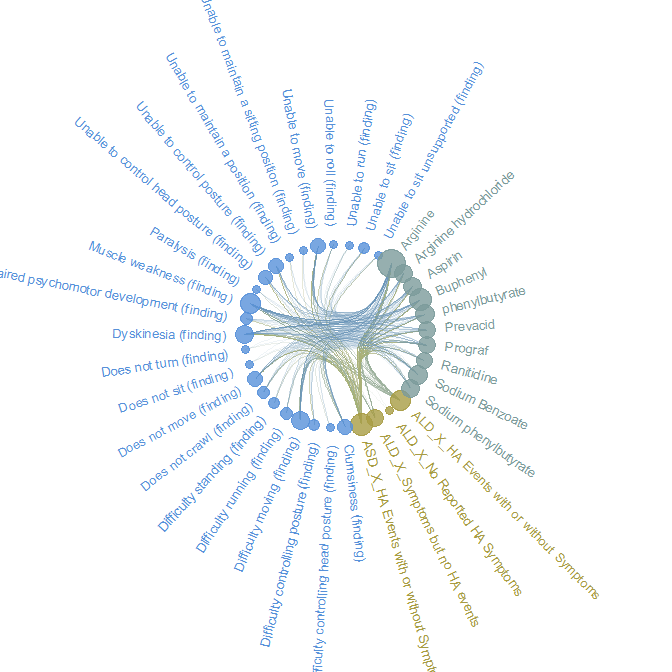
\includegraphics[width=4.5in]{EdgeBundle2.png}}
    \centering
    \caption{UCD radial edge bundled graph with Nodes Sized for n, and Node Labels, and Edges Colored by Node Type}
    \label{fg:edgebund2}
\end{figure}

\subsection{Hiearchical Dendrogram with Nodes, Labels, and Edges}

Script:
\small
\begin{verbatim}
                ggraph(g, layout='dendrogram', circular=F) +
                  # Coordinates:
                  # Plot extents are (0,0) to (n_leaves-1,n_levels-1), where n_levels is the number of levels
                  # in the hierarchy (one for origin to origin, one for the groups with from="origin," and one
                  # for leaves)
                  # leaves are placed at x=0..n_leaves-1, y=0
                  # Draw arcs first, so that points overlay ends
                  geom_edge_diagonal(alpha=0.5) +
                  # x, y coordinates are generated by ggraph() (use str(ggraph(...)) to review elements)
                  # from and to are taken from the edge data frame
                  geom_conn_bundle(data=get_con(from=edge[,"from"], to=edge[,"to"], v12=edge[,"v12"]),
                    aes(x=x, y=y, color=v12), edge_width=0.35, alpha=0.1, tension=0.75) +
                  scale_edge_color_manual(values=ecolor, guide=F) +
                  # v and n are taken from the vertex data frame used to construct g
                  geom_node_point(aes(x=x, y=y, size=n,
                    color=ifelse(v!="origin", v, ifelse(name!="origin", name, "Participants")))) +
                  geom_node_text(aes(x=ifelse(v!="origin", x, x+1),
                                     y=ifelse(v!="origin", y-0.2, y),
                  label=ifelse(name!="origin", name, "Participant"),
                    color=ifelse(v!="origin", v, ifelse(name!="origin", name, "Participants")),
                    angle=ifelse(v!="origin", 90, 0),
                    vjust=0.5,
                    hjust=ifelse(v!="origin", 1, 0),
                    # Note that node and text sizes are from disjoint spaces, but ggplot does not
                    # support multiple scale_size functions
                    # Therefore, scale text the range of point sizes, which are based on participant
                    # counts
                    size=ifelse(v!="origin", 10, ifelse(name!="origin", 20, 30)))) +
                  scale_color_manual(values=setNames(c("black",
                    rgb(matrix(col2rgb("#FFEE66"), nrow=1)/390),
                    rgb(matrix(col2rgb("#66AAFF"), nrow=1)/300),
                    rgb(matrix(col2rgb("#88AAAA"), nrow=1)/280)), c("Participants", v)),
                    guide=F) +
                  #scale_size_manual(values=c("t1"=3, "t2"=4, "t3"=5), guide=F) +
                  expand_limits(x=c(NA, length(which(h[,"from"]!="origin"))+5), y=c(-2.5, NA)) +
                  theme_void() + theme(plot.margin=margin(0.25, 0.25, 0.25, 0.25, "in"))
\end{verbatim}
\normalsize

Result:

\begin{figure}[H]
    \frame{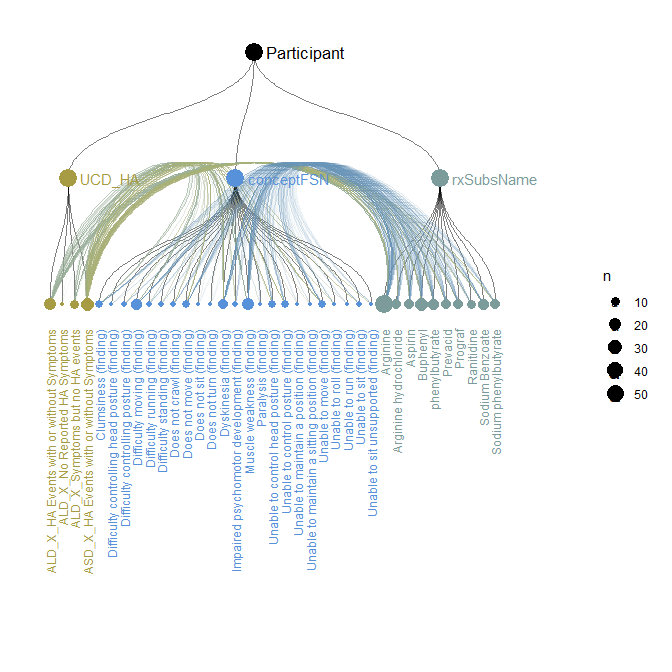
\includegraphics[width=4.5in]{Dendrogram4.png}}
    \centering
    \caption{Hierarchical UCD dendrogram with edges relating nodes by participant}
    \label{fg:edgebund4}
\end{figure}

%%%%%%%%%%%%%%%%%%%%%%%%%%%%%%%%%%%%%%%%%%%%%%%%%%%%%%%%%%%%%%%%%%%%%%%%%%%%%%%%%%%%%%%%%%%%%%

\section{Debugging}\label{sec:debugging}

It is important that you have a means of communicating with your app during execution.  Unlike a typical R script, that can be executed one line at a time, with interactive review of variables, once a Shiny script launches, it executes without the console prompt.  Upon termination, some global variables may be available for examination, but you may not have reliable information on when they were last updated.  Error and warning messages are displayed in the console (and the terminal session when executed in a shell) and, fortunately, so are the results of \texttt{print()} and \texttt{cat()}.  When executed in RStudio, Shiny offers sophisticated debugger features (more info at \url{https://shiny.rstudio.com/articles/debugging.html}).  However, one of the simplest methods of communicating with your app during execution is to use \texttt{print()} (for a formatted or multi-element object, such as a data frame) or \texttt{cat(, file=stderr())} for ``small" objects.  The \texttt{file=stderr()} causes displayed items to appear in red.  Output may also be written to an error log, depending on your OS.  Considerations include

\begin{itemize}
    \item Shiny reports line numbers in error messages relative to the related function (\texttt{ui()} or \texttt{server()}) and, although not always exact, reported lines are usually in the proximity of the one which was executed at the time of error
    \item \texttt{cat("your message here")} displays in RStudio console (generally, consider Shiny Server)
    \item \texttt{cat("your message here", file=stderr())} is treated as an error (red in console, logged by OS)
    \item Messages appear in RStudio console when Shiny app launched from within RStudio
    \item Messages appear in terminal window when Shiny app launched with the \texttt{rscript} command in shell
    \item There exists a ``showcase" mode (\texttt{runApp(display.mode="showcase")}) that is intended to highlight each line of your script as it is executing
    \item The reactivity log may be helpful in debugging reactive sequencing issues (\texttt{options(shiny.reactlog=T)}, \url{https://shiny.rstudio.com/reference/shiny/0.14/showReactLog.html}
    \url It may be helpful to initially format an apps appearance with an empty \texttt{server()} function, then include executable statements once the screen objects are available and configured
    \item Although not strictly related to debugging, the use of \texttt{gc()} to clear defunct memory (from R's recycling) may reduce total memory in use at a given time
\end{itemize}


\end{spacing}

\end{document} 